\documentclass[a4paper,12pt,release]{article}

\title{AnimEditor használati útmutató}
\date{Frissítve: 2020.02.17.}

\def\magyarOptions{defaults=hu-min}
\usepackage[utf8]{inputenc} %Tudok ékezetes karaktereket írni
\usepackage[T1]{fontenc} %Ez talán a babelnek kell...
\usepackage[bottom,flushmargin,stable]{footmisc} %A footnote-kat szépíti
\usepackage[magyar,english]{babel} %Szótagol
\usepackage{indentfirst} %Az első bekezdést behúzza
\usepackage{graphicx} %Képeket lehet betenni
\usepackage{wrapfig} %Képaláírásokat és körbefuttatást kezel
\usepackage{anysize} %Margókat kezel
\usepackage{setspace} %Sorközöket kezel
\usepackage{multicol} %hasábol
\usepackage{hyperref}
\usepackage{titling}
\renewcommand\maketitlehooka{\null\mbox{}\vfill}
\renewcommand\maketitlehookd{\vfill\null}

\addto\captionsenglish{
	\renewcommand{\contentsname}%
	{Tartalom}%
}

%-------------------------------------------------------------------------------
\marginsize{1cm}{1cm}{0cm}{1cm}
%-------------------------------------------------------------------------------
\begin{document}
\maketitle
\newpage
\tableofcontents
\clearpage
\section{Gyors referencia}
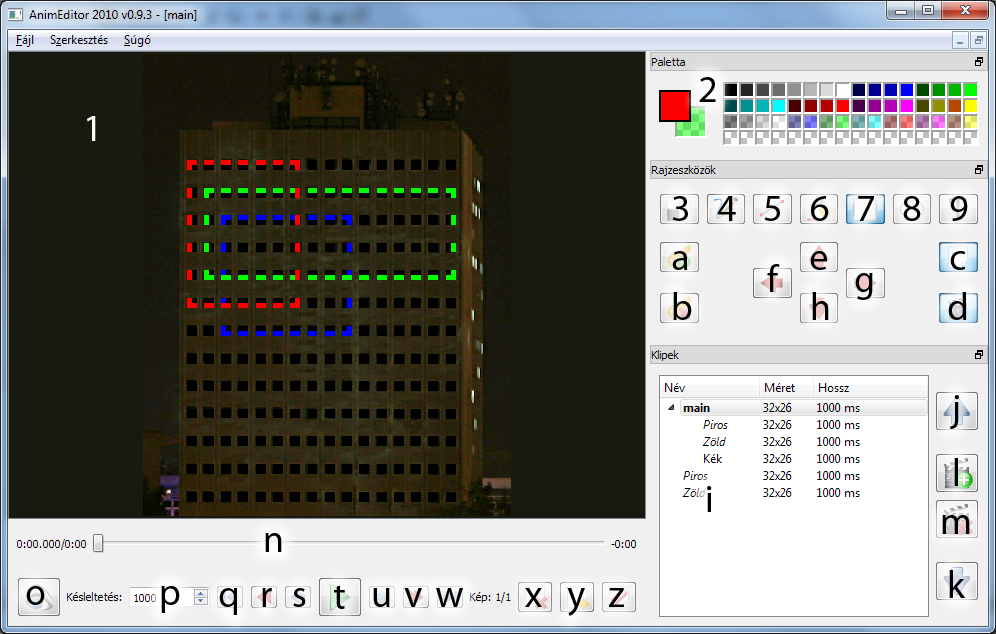
\includegraphics[width=0.9\textwidth]{pics/main.jpg}\\
\begin{multicols}{3}
\begin{itemize}
\item[1]Szerkesztőfelület
\item[2]Paletta
\item[3]Pixel/ablakválasztó
\item[4]Ceruza
\item[5]Vonal
\item[6]Kifestő
\item[7]Téglalap
\item[8]Ellipszis
\item[9]Szöveg
\item[a]Keyframe beszúrása
\item[b]Keyframe eltávolítása (ha van)
\item[c]Rajz mozgatása (kapcsológomb)
\item[d]Beágyazott klipek mozgatása (kapcsológomb)
\item[e]Mozgatás felfelé 1 ablakkal
\item[f]Mozgatás balra 1 ablakkal
\item[g]Mozgatás jobbra 1 ablakkal
\item[h]Mozgatás lefelé 1 ablakkal
\item[i]Klipek és beágyazás
\item[j]Takarási sorrendben felfele mozgatás
\item[k]Takarási sorrendben lefele mozgatás
\item[l]Új beágyazott klip felvétele a kijelölthöz
\item[m]Kijelölt klip eltávolítása
\item[n]Időcsúszka
\item[o]Beágyazott klipek mutatása/elrejtése
\item[p]Aktuális képkocka hossza
\item[q]Legelső képkockára ugrás
\item[r]Előző keyframe-re ugrás
\item[s]Előbő képkockára lépés
\item[t]Lejátszás/megállítás
\item[u]Következő képkockára lépés
\item[v]Következő keyframe-re ugrás
\item[w]Utolsó frame-re ugrás
\item[x]Épp mutatott képkocka törlése
\item[y]Aktuális képkocka megkettőzése
\item[z]Aktuális képkockán levő rajz eltávolítása
\end{itemize}
\end{multicols}
\clearpage
\section{Az AnimEditor használata}
Az első oldalon megtalálható a gombok rövid leírása, ezt nem árt magadnál tartani olvasás közben. A program használata közben azonban nem kell egyfolytában ide visszajönnöd, ugyanis minden gombhoz tartozik tooltip, mely emlékeztet a gomb funkciójára.

Az ablak két nagy részből épül fel, az egyik a rajzfelület (1), a másik minden más :). A panelek elrendezése variálható, ha nem tetszik az alapállapotuk, húzd őket máshova -- akár a főablakon kívülre is!

Röviden összefoglalva úgy kell használni a programot, hogy kiválasztasz egy rajzeszközt, és rajzolgatsz az egyik rajzfelületre \`a la Paint. Készíthetsz klipeket is, ezeket korlátlanul beillesztheted más klipekbe, vagy közvetlenül az animációba (ismétlődő motívumok esetén -- pl. refrén -- ez különösen hasznos lehet).

\subsection{Argumentumok}
\begin{description}
\item[-sideaudio] Automatikusan betölti a .qp4/.q4z-nek megfelelő nevű hangfájlt, ha talál olyat mellette.
\item[-english] Angol nyelvű módban indítja el a programot.
\end{description}

\subsection{Rajzeszközök}
\begin{wrapfigure}{r}{0.5\textwidth}
	\vspace{-27pt}
	\begin{center}
		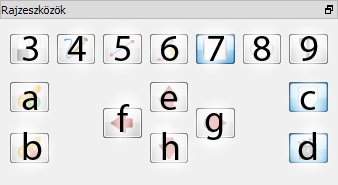
\includegraphics[width=0.5\textwidth]{pics/tools.png}
	\end{center}
	\vspace{-20pt}
\end{wrapfigure}
A rajzeszközök alapértelmezettként a program jobb oldalán, középen találhatóak meg. Itt tudod kiválasztani, hogy mit csináljon egy rajzfelületre történt kattintás (3-9 gombok), illetve tudod a látott képet egy ablaknyival arrébtolni (e-h és c,d gombok). A bal gomb az előtér-, a jobb gomb a háttérszínnel rajzol, fest, stb. Az animációkezelés is részben itt van, az a,b gombokkal tudsz keyframe-et betenni vagy kivenni (főleg kivenni, mivel a beágyazott klipek mozgatása automatikusan keyframe-et hoz létre).

\subsection{Rajzeszközök (4-9)} Ezek kapcsológombok (egyszerre csak egy lehet aktív). A rajzolás a klipre történik, a beágyazott klipekre nincs hatással!
\begin{description}
\item[Pixelméret (3)]Beállítható, hogy a rajzeszközök pixeleken vagy ablakokon dolgozzanak.
\item[Ceruza (4)]Szabadkézi rajzolást tesz lehetővé.
\item[Vonal (5)]Egyenes vonal húzása: a vonal kezdeténél nyomd le a kívánt egérgombot, húzd el a kurzort a vonal végéhez, majd engedd el a lenyomott egérgombot!
\item[Kifestés (6)]Egy pixelre kattintva a körülötte levő vele azonos színű pixeleket a kattintásnak megfelelő színre cseréli (leánykori nevén floodfill).
\item[Téglalap (7)]Működése hasonló a vonaléhoz, de a két pont egy téglalap két sarkát jelöli ki. A téglalap kerete a kattintásnak megfelelő színű lesz, a belseje a másik egérgombénak.
\item[Ellipszis (8)]Mint a téglalap, de téglalap helyett beleírt ellipszist rajzol.
\item[Szöveg (9)]Használatakor elég rákattintani a kívánt rajzfelületre. A kattintás után megjelenik egy párbeszédablak, melyben megadható a betűtípus, a szöveg, és a szöveg beúszásának ideje ideje. A szöveg külön klipként fog beágyazódni.
\end{description}
\subsubsection{Téglalap (7) és ellipszis (8) eszközök}
Ezeknél az eszközöknél kétféle átlátszóságot különböztet meg a program. Az RGBA 0,0,0,0 töltőszín azt okozza, hogy az alakzat belseje nem lesz kifestve (tehát csak a kerete lesz megrajzolva), minden egyéb 0 alfa-értékű szín (pl. 255,0,0,0) pedig átlátszó színnel rajzolja át az alakzat belsejét (``ablakot'' nyitva ezzel a beágyazott klipeknek). Segítségképp a paletta alsó sorának második színe egy ilyen szín.
\subsubsection{Szöveg eszköz (9)}
\begin{wrapfigure}{r}{0.5\textwidth}
	\vspace{-27pt}
	\begin{center}
		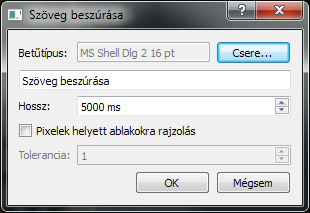
\includegraphics[width=0.5\textwidth]{pics/inserttext.png}
	\end{center}
	\vspace{-20pt}
\end{wrapfigure}
A szöveg eszköz picit máshogy működik, mint a többi rajzeszköz. Először is, mindegy, hogy hova kattintasz az ablakon, mert a szöveg klipként kerül be. Másodszor pedig külön beállítóablaka van (ábra jobboldalt).

Az ablakban meghatározhatod a betűtípust, a megjelenítendő szöveget, a szöveg képernyőn átfutásának idejét, illetve kérheted, hogy a szöveg ne pixelekre, hanem ablakokra rajzolódjon. Az ablakokra rajzolt eredmény nagyon függ a használt betűtípustól, illetve betűmérettől, valamint a toleranciaérték változtatásától (0-4 között lehet).

Az OK gomb lenyomására egy klip kerül a választott klipedbe, mely szintén klipként tartalmazza az egész szöveget (keyframe-ekkel lehet a szöveg beúszását módosítani, pl. pattogó szöveget készíteni).

\subsubsection{Animációs eszközök}
Ezek a már megrajzolt képek időbeni viselkedését módosítják. Az aktuálisan aktív klipablakra fejtik ki hatásukat, aktuális időponton a klipablakban található csúszka (n) által meghatározott időpontot értjük.

Keyframe-nek nevezünk egy olyan időpontot, melyben rögzítve vannak a klipek helyei (pl. klip beszúrása keyframe, vagy az e-h gombok lenyomásakor is automatikusan keyframe jön létre). A keyframe-ek között a pozíciók lineárisan interpolált értéket vesznek fel.
\begin{description}
\item[Keyframe felvétele (a)]{Rögzíti a beágyazott klipek pozícióját az aktuális időpontban.}
\item[Keyframe eltávolítása (b)]{Ha az aktuális időpontban van keyframe, eltávolítja azt, a beágyazott klipek a környező két keyframe által meghatározott pozíciót veszik fel. Keyframe-ek kereséséhez használd az r,v gombokat!}
\item[Rajzolás mozgatása (c)]{Ha ez a gomb le van nyomva, a mozgatógombok (e-h) a rajzolt képet (is) mozgatják. {\bf Vigyázat!} A rajz mozgatásakor a klip széléről kimozgatott pixelek elvesznek!}
\item[Beágyazott klipek mozgatása (d)]{Ha le van nyomva, az e-h mozgatógombok a beágyazott klipeket (is) mozgatják. Ha beágyazott klipet mozgatsz ki a képből, nem vesznek el pixelek.}
\item[Mozgatás (e-h)]{A c és d gombok által meghatározott dolgot mozgatja a gomb ikonjának megfelelő irányba egy ablaknyival (2 pixel). Ha szeretnéd, hogy a klip ``ugorjon'', az előző pillanatban vegyél fel egy keyframe-et még a mozgatás előtt, különben lineárisan fog mozogni!}
%redundancia by Vandra Ákos ^^^^^^^^^^
\end{description}
\clearpage
\subsection{Paletta}
\begin{wrapfigure}{r}{0.5\textwidth}
	\vspace{-27pt}
	\begin{center}
		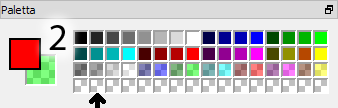
\includegraphics[width=0.5\textwidth]{pics/palette.png}
	\end{center}
	\vspace{-20pt}
\end{wrapfigure}
Itt lehet megadni a színeket. Színkeverésnél a teljes RGBA8888 színtér rendelkezésedre áll, de ne feledd, hogy a Mátrix az RGB333 színtért képes megjeleníteni. Segítségként a Schönherz képén levő animáció már kerekített színekkel jelenik meg (egyéb klipeknél nem).

Ha bal egérgombbal rákattintasz a jobboldali részen egy színre, az a baloldalt kijelölt színt leváltja (baloldalt szín kijelölése szintén bal klikkel történik). Jobb kattintással megnyithatod a színkeverő ablakot, melyben új színt adhatsz meg. A pepitaminta az átlátszóság szemléltetésére szolgál (alapértelmezettként a legalsó sor teljesen átlátszó színeket tartalmaz).

A baloldalt fent található szín (a képen piros) a bal egérgombhoz, az alatta található (a képen átlátszó zöld) a jobb egérgombhoz van rendelve rajzoláskor.

A nyíllal jelölt szín teljesen átlátszó, de a téglalap (7) és ellipszis (8) eszközök kitöltik a rajzolt alakzatot ezzel a színnel.

\subsection{Klipek}
\begin{wrapfigure}{r}{0.5\textwidth}
	\vspace{-27pt}
	\begin{center}
		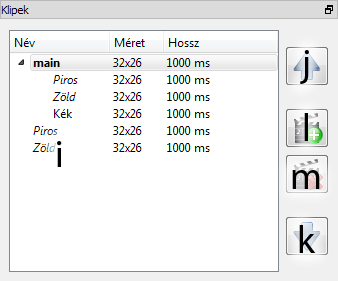
\includegraphics[width=0.5\textwidth]{pics/library.png}
	\end{center}
	\vspace{-27pt}
\end{wrapfigure}
Itt találhatóak meg az animációban levő klipek, a beágyazás szerinti fastruktúrába rendezve. Az első oszlopban a klip nevét láthatod,
\begin{description}
\item[Sima betűvel,]ha a klip nincs beágyazva több helyre,
\item[\emph{Dőlt betűvel,}]ha a klip több helyre is be van ágyazva,\\
illetve a {\bf ``main''} mindig vastag betűvel van írva.
\end{description}

A {\bf main} klip maga az animációd, ezt fogjuk levetíteni a Schönherz falán. Különleges bánásmódban részesül, pl. más rajzterülete van, illetve nem ágyazható be sehova (viszont másolatot lehet róla készíteni).

A beágyazás a modellezőprogramokhoz hasonlóan működik: ha egy dőlt betűs klipet módosítasz, minden előfordulása módosulni fog. Ha nem szeretnéd ezt, kattints jobb gombbal a megfelelő klipre, és válaszd ki a Leválasztás menüpontot. A leválasztott klip új nevet kap, és külön szerkeszthető.

A második és harmadik oszlop reméljük, magától értetődik: a második oszlop a klip méretét (szélesség x magasság) adja meg pixelekben (negyed ablak), a harmadik pedig a klip hosszát ezredmásodpercben.

\begin{wrapfigure}{r}{0.4\textwidth}
	\vspace{-27pt}
	\begin{center}
		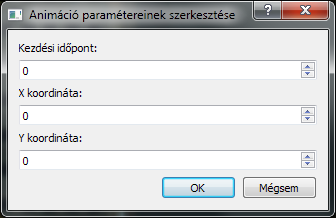
\includegraphics[width=0.4\textwidth]{pics/childsettings.png}
	\end{center}
	\vspace{-27pt}
\end{wrapfigure}
A klipek a listában levő sorrendjük alapján takarják el egymást rajzoláskor (a listában előrébb levő eltakarja az utána levőt, valamint a tartalmazó klip képkockái eltakarják a tartalmazott klipeket). A sorrend megváltoztatására a j és k jelzésű gombok szolgálnak.

Az l és m gombok a jobbklikkes menü megfelelő menüpontjainak felelnek meg: az l új klipet ágyaz be a kijelölt klipbe, az m pedig eltávolítja a kijelölt klipet.

A klipek jobb-klikkes menüjében külön említést érdemel a Paraméterek menüpont. Itt beállíthatod, hogy a klip mikor kezdődjön a szülőjében (időbeli ``eltolást'' csak ilyen módon lehet megtenni beágyazás után), illetve megadhatod a beágyazás helyét. Az itt beállított koordináták eltolják az összes keyframe-et is, ez szintén hasznos lehet.

\section{Animációkezelés}
\begin{wrapfigure}{r}{0.75\textwidth}
	\vspace{-27pt}
	\begin{center}
		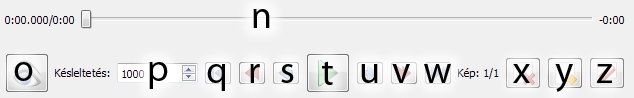
\includegraphics[width=0.75\textwidth]{pics/timeline.png}
	\end{center}
	\vspace{-27pt}
\end{wrapfigure}
Ez a panel minden animáció ablakában megtalálható. Itt lehet képkockákat felvenni, illetve a már meglévők között lépkedni. A w és x gombok között láthatod, hogy épp hanyadik képkockán állsz (aktuális/összes alakban). Ha az aktuális képkocka ``-{}-'', az utolsó képkocka után állsz (ilyenkor nem tudsz rajzolni, hiszen nincs is mire). A kezelőszervek működése:
\begin{description}
\item[Idővonal (n)]Ennek használatával tetszőleges időpontra ugorhatsz -- 20 ms-os léptékben. Baloldalt perc:másodperc.ezred/perc:másodperc alakban láthatod a pozíciódat/a klip hosszát, jobboldalt pedig az aktuális pozíciótól a klip végéig hátralevő időt.
\item[Beágyazott klipek mutatása/elrejtése (o)]Kapcsológomb, segítségével elrejtheted a beágyazott klipeket. Ez a funkció csak a szerkesztést segíti, a mentett fájlban (és a Mátrixon is) minden mutatva lesz. Ha nem szeretnéd, hogy egy klip látszódjon a Mátrixon, távolítsd el!
\item[Késleltetés (p)]Itt megadhatod, hogy az épp mutatott képkocka mennyi ideig látszódjon -- szintén 20 ms-os léptékben.
\item[Visszatekerés (q)]A klip legelejére ugrik.
\item[Előző keyframe-re ugrás (r)]Az előző keyframe-re ugrik -- ha van olyan.
\item[Előző képkockára lépés (s)]Az előző képkockára lép.
\item[Lejátszás/megállítás (t)]Lejátssza/megállítja az animációt. A {\bf main} esetében ha van megadva hangfájl, az is hallható lejátszás közben.
\item[Következő képkockára lépés (u)]A következő képkockára lép.
\item[Következő keyframe-re ugrás (v)]A következő keyframe-re ugrik -- ha van olyan.
\item[Előretekerés (w)]A klip legvégére ugrik.
\item[Képkocka törlése (x)]Eldobja az aktuális képkockát. Nem lehetséges 0 méretű klipet létrehozni, ha kitörlöd az összes képkockát, beszúródik egy automatikusan.
\item[Képkocka megkettőzése (y)]Az aktuális képkocka után elhelyezi annak másolatát.
\item[Rajz törlése (z)]Az aktuális képkockán található rajzot kitörli, csak a beszúrt klipek látszódnak (ha vannak).
\end{description}
\section{A menük}
Három menü van: Fájl, Szerkesztés és Súgó. A súgóban mindössze a program névjegyét tekintheted meg, a szerkesztésben pedig a csapatod információit adhatod meg. Ezt kérjük, tedd meg!

A Szerkesztés menüben található még egy másolás/beillesztés funkció, ezzel azonos méretű klipek között tudsz képeket másolni. A beillesztés mindig az éppen mutatott képkocka után teszi be a képet.

A Fájl menüben betölthetsz idei (QP4 vagy Q4Z) animációt, illetve importálhatsz régi QPA animációt is.

A QP4 egy új szöveges formátum (leírása a függelékben), vele ekvivalens a Q4Z, mely QP4 fájlt tartalmaz tömörítve.

Szintén a Fájl menüben lehetőséged van hang hozzárendelésére az animációdhoz (MP3 vagy OGG formátumban).
\section{Az animációk beadása}
Az animációkat a Qpahonlapon megadott módon és helyre kell feltölteni. Győződj meg róla, hogy megfelelő hangfájlt töltöttél be, nézd végig az animációdat, és ha mindent rendben találsz, a {\bf Fájl} menüből válaszd az {\bf Exportálás beküldésre} funkciót. Az elmentett .q4x fájlban megtalálható a hang is, így elég csupán ezt a fájlt feltölteni.
\clearpage
\section{Függelék: A QP4 formátum}
A QP4 formátum sokkal többet tud a régi QPA formátumnál, ugyanis programnyelv! :)

Egész pontosan a QP4 fájlok UTF-8 kódolású Lua\footnote{A Lua letölthető innen: \href{http://www.lua.org}{http://www.lua.org}} szkriptek (a \foreignlanguage{english}{World of Warcraft}-ból ismerős lehet, ott ilyen nyelven készülnek az addonok).

Kétféle leírást közlünk a QP4-hez, először azoknak, akik pusztán átkonvertálni szeretnék animációikat, majd azoknak, akik le is szeretnék programozni.

\subsection{QP4 konvertálásra}
Az első sorban add meg a csapatod adatait, illetve a használni kívánt hangfájl lokális elérhetőségét ilyen formában:
\\\\
meta(\{team="Csapatnév",title="Animáció címe",year=2011,audio="/home/neo/music.ogg"\})
\\\\
Értelemszerűen az adatokat behelyettesítve.
A következő sor ez legyen:
\\\\
beginclip(32,26,"main")
\\\\
Ezután felsorolhatod az animációd képkockáit, így:
\\\\
frame(\{pixelek\},20)\\
frame(\{pixelek\},20)\\
-{}- satöbbi
\\\\
Ahol pixelek egy 32*26=936 méretű, vesszővel elválasztott 0xAARRGGBB alakú pixeltömb. A pixelek balról jobbra, soronként fentről lefele olvasódnak ki. A frame második paramétere a képkocka hossza, ezredmásodpercben. Javasoljuk, hogy 20 ms többszörösét add meg itt. Ne feledd, hogy a megadott színeket kerekítjük a Mátrix által megjelenített színekre, a fájlt nézd meg az AnimEditorban is!

Az utolsó képkocka után ezt írd a fájl végére:
\\\\
endclip()\\
rootclip("main")
\\\\
Kész is vagy. A biztonság kedvéért nézd meg az AnimEditorban is az animációt, mielőtt exportálod!
\clearpage
\subsection{QP4 programozóknak}
A QP4 Lua 5.3.5-el fut. A Luát update-eltem 5.3.5-re a 2012-es állapothoz képest, ez a bit32 libraryt megszünteti, ami eltörhet egyes régi animációkat. A Q4X formátum ezért verziót lépett 2-re.
\\
\\Ez egy lehetséges workaround régi animációkhoz, ha berakod a .qp4 elejére:
\begin{verbatim}
local bit32 = bit32 or load([[return {
band = function(a, b) return a & b end,
bor = function(a, b) return a | b end,
bxor = function(a, b) return a ~ b end,
bnot = function(a) return ~a end,
rshift = function(a, n) return a >> n end,
lshift = function(a, n) return a << n end,
}]])()
\end{verbatim}
Fontos újítása az 5.2-nek, hogy függvényenként már $2^{26}$ konstans áll rendelkezésre, illetve már beépítve is találhatóak bitműveletek. Rendelkezésedre állnak a base, package, coroutine, table, string, math könyvtárak.
A következő globális függvényekkel kapcsolódhatsz az AnimEditorhoz:
\begin{description}
\item[debug(string)]A paraméterként átadott stringet megjeleníti betöltés után ({\bf Vigyázat!} Sok debug()-hívás nagyon lassú is lehet!)
\item[meta(table)]Megadja a csapatinformációkat. A table kulcsai: "audio" => hangfájl, "team" => csapatnév, "title" => animáció címe, "year" => évszám. A year szám, minden más szöveg típusú. Nem kötelező mindet megadni, sőt, akár több meta() hívással is megadhatóak az információk.
\item[beginclip(width,height,name)]Új klipet készít, width*height mérettel (pixelben), "name" névvel. Width, height szám típusú, name egy string. A klip méreteinek párosnak kell lenniük. A klip lezárása az endclip() függvénnyel történik, klipek így nem ágyazhatóka egymásba (arra az embed() való).
\item[frame(pixels,delay)]Új képkockát szúr be a megnyitott klipbe. A pixels egy width*height méretű számtömb, részletesen lásd az előző szakaszban. A delay a kép hosszát adja meg ezredmásodpercben. Javasoljuk, hogy legyen 20 egész számú többszöröse.
\item[embed(name,x,y,z,t)]A "name" nevű klipet beszúrja z Z-indexszel, t időpontban. A "name" klipnek már léteznie kell. A z-index jelenleg nem használt, a Z-ordert a beszúrások sorrendje határozza meg. x és y táblázat, a kulcsa egy időpont (t-hez képest), értéke pedig egy szám -- itt adod meg a keyframe-eket (a nem megadott időpontok között lineárisan interpolálódik a koordináta). Javasoljuk, hogy adj meg 0 kulcsot.
\item[endclip()]Lezárja az adott klipet. Csak beginclip()-pel párban használható.
\item[rootclip(name)]A megadott klipet elhelyezi a legfelső szinten (a main mellett). A main-t fel kell venni rootclip()-pel. Betöltés után a rootclipekből nem elérhető klipek eldobásra kerülnek.
\\\\
Mellékeltünk egy példa QP4 fájlt example.qp4 néven, illetve az AnimEditor mentéskor a debug() kivételével minden függvényt használ, onnan is lehet példákat nézni.
\end{description}
\end{document}